\documentclass[11pt]{article}
\usepackage{graphicx}
\usepackage{array}
\usepackage{booktabs}
\usepackage[a4paper,margin=3cm, headheight=90pt]{geometry}
\usepackage{cmbright}
\usepackage[OT1]{fontenc}
\usepackage{float}
\usepackage[table]{xcolor}
\usepackage{pgfplots}
\pgfplotsset{compat=newest}
\usepackage{caption}
\usepackage{subcaption}
\usepackage{fancyhdr}
\usepackage{blindtext}
\usepackage{natbib}
\setcitestyle{square}
\usepackage{url}
\usepackage{wrapfig}
\usepackage{amsmath}
\usepackage{parskip}
\usepackage{tabularx}
\newcolumntype{Y}{>{\centering\arraybackslash}X}
\usepackage{multirow}

\title{\vspace{-2cm}
\includegraphics[width=0.3\textwidth]{/Users/finn/Documents/Cardiff-University-logo-for-website}~\\[1cm]
Title
}
\author{Finnbar Wilson - 22031076}
\date{\today}

\begin{document}

\maketitle

\section*{Abstract}

\pagebreak
\section{Introduction}

NGC 3201 is a globular cluster, discovered by James Dunlop on the 28th of May 1826, located at 10$^{\text{h}}$ 17$^{\text{m}}$ 36.82$^{\text{s}}$/-46$^{\circ}$ 24' 44.9" (in RA/Dec) 5.0 kpc away from the Sun \citep{3201fact}. NGC 3201 has a large sub-cluster of black hole in its core making it an interesting source for observing the interactions in large populations of black holes \citep{blackholes}.

Globular clusters are among the oldest stellar populations in the universe, providing key insights into how stars and galactic structures evolve. In the Milky Way, some clusters are thought to have originated outside the galaxy due to their similar properties to satellite dwarf galaxies, whereas others are believed to have evolved within the milky way itself due to the observable effects of tidal forces and shocks in the inner galaxy. This allows for globular clusters to be classified by their characteristics as shown by \citet{Mackey} into three types: 'Young' halo(YH) which are thought to have been formed in external galaxies, 'Old' halo(OH) and 'Bulge/Disc'(BD) which are formed in the milky way. According to \citet{Mackey}, their study on globular clusters classified NGC 3201 as a YH cluster based on the metallicity and redder horizontal branch stars. NGC 3201 stands out from other clusters classified by \citet{Mackey} due to its irregular radial velocity and differential reddening across its face \citep{Kravtsov}. This makes it one of the few known clusters with an inhomogeneous stellar population for its size, which could affect how it has been classified.

In this report the structure of NGC 3201 will be analysed by finding the stellar populations inside the cluster and comparing them to isochrones to determine their age. These stellar populations will then allow a greater insight into the internal structer of the cluster creating a more actuate annalysis of its classification. Given that NGC 3201 is an abnormal cluster this report will also test various methods of determining the classification of abnormal clusters.

\section{Procedure}

\subsection{Calibration}

Two images of NGC 3201 were taken in the V and B filters on a 1.0m diameter telescope. Five stars were found in each filter to calibrate the zero point magnitude in each image and their data can be found in Table \ref{tab:calB} \& \ref{tab:calV}. To find the calibration stars a catalog of local stars from \citet{simbad} was overlaid in each image and 10 stars were selected in total and their known magnitudes recored. An apature photometery of each star was performed and recorded as well as their error.

\begin{table}[H]
\centering
\caption{Calibration stars in B filter}
\begin{tabular}{lccccc}
\toprule
ID & RA & Dec & B$_{\text{instrument}}$ & B$_{\text{simbad}}$ \\
\midrule
Cl* NGC 3201 CWFD 3-109 &  10:17:23.65 &  -46:24:17.31 & -12.566$\pm 0.004$ & 16.216 \\                  
Cl* NGC 3201 CWFD 3-198 &  10:17:34.49 &  -46:25:36.15 & -12.947$\pm 0.003$ & 15.800 \\                 
Cl* NGC 3201 CWFD 3-224 &  10:17:36.86 &  -46:23:11.97 & -15.062$\pm 0.001$ & 13.601 \\                 
NGC 3201 3401 &  10:17:38.12 &  -46:22:39.29 & -14.787$\pm 0.001$ & 14.080 \\                           
NGC 3201 4319 &  10:17:42.55 &  -46:27:15.42 & -14.812$\pm 0.001$ & 13.999 \\
\bottomrule
\end{tabular}
\caption*{ID is the stars identifcation searchable on the SIMBAD database, B$_{\text{instrument}}$ is the magnitude recorded in this experiment and B$_{\text{simbad}}$ is the known magnitude found on SIMBAD \citep{simbad}}
\label{tab:calB}
\end{table}

\begin{table}[h]
\centering
\caption{Calibration stars in V filter}
\begin{tabular}{lcccccc}
\toprule
ID & RA & Dec & V$_{\text{instrument}}$ & V$_{\text{simbad}}$\\
\midrule
2MASS J10173339-4620241 & 10:17:33.39 & -46:20:24.16 & -13.579$\pm 0.003$ & 15.650 \\                   
Cl* NGC 3201 CWFD 3-296 & 10:17:42.26 & -46:19:47.92 & -13.904$\pm 0.002$ & 15.230 \\                  
Cl* NGC 3201 CWFD 3-255 & 10:17:38.86 & -46:22:56.86 & -14.536$\pm 0.002$ & 14.730 \\                  
Cl* NGC 3201 CWFD 3-235 & 10:17:37.72 & -46:22:53.50 & -14.410$\pm 0.002$ & 14.910 \\                     
Cl* NGC 3201 CWFD 3-195 & 10:17:34.01 & -46:23:26.20 & -13.225$\pm 0.003$ & 16.030\\ 
\bottomrule
\end{tabular}
\caption*{ID is the stars identifcation searchable on the SIMBAD database, V$_{\text{instrument}}$ is the magnitude recorded in this experiment and V$_{\text{simbad}}$ is the known magnitude found on SIMBAD \citep{simbad}}
\label{tab:calV}
\end{table}

The equation to find the zero point magntidue is shown by Equation \ref{eq:zp}.
\begin{equation}
	m_{\text{zero point}} = m_{\text{simbad}} - m_{\text{instrument}}
	\label{eq:zp}
\end{equation}
Where $m$ is the magnitude (B or V). This produced a zero point magnitude of: B$_{\text{zero point}} = 28.774 \pm 0.005$ and V$_{\text{zero point}} = 29.2407 \pm 0.0010$. The errors associated with these values are from the error in the $m_{\text{instrument}}$ recordings as well as the error in the $m_{\text{simbad}}$ which are not shown in Table \ref{tab:calB} \& \ref{tab:calV} but can be found on \citet{simbad}. 

\subsection{Automated detection}

An object detection tool from \citet{gaia} was used to quickly identify the magnitudes of large number of stars in each image as well as their positions and information on how they selected those stars. These two large datasets were then uploaded into \citet{topcat} which matched the two filters by their positions so that the magnitudes recorded are for the same stars. This matched dataset can be found on the \citet{github}. The automated object detection tool found it hard to indentify singular stars in the dense core so other detection methods are needed to annalyse the centeral stars of the cluster. This tool was able to calulate the error in both magnitudes. this method records magntiude as apparent magnitude so to convert it into Absolute magntiude Equation \ref{eq:absolute} can be used.
\begin{equation}
	m-M = 5 \log \left( \frac{d}{10} \right)
	\label{eq:absolute}
\end{equation}
Where $m$ is the apparent magntiude, $M$ is the absolute magntiude and $d$ is the distacne to NGC 3201.
\subsection{Manual detection}

An apature photometry tool was used to manually determine the magniude of stars foucsing especially around the core where the automated detections system found it harder to detect stars. Stars were chosen based on their shape, to ensure only that star was being recored instead of multiple, as well as theri brighness. This tool was able to calulate the error in the magnitude data for both filters.

\section{Analysis}

\subsection{Determing age of NGC 3201}

The matched data from the automated detection method is shown in Figure \ref{fig:origin}. The matched dataset orignally recored 7612 stars but this number was reduced to 2411 stars by removing stars that lay outside of 0.152$^{\circ}$ from the center of the cluster as this is the radius of NGC3201 \citep{radius}. 

\begin{figure}
	\centering
	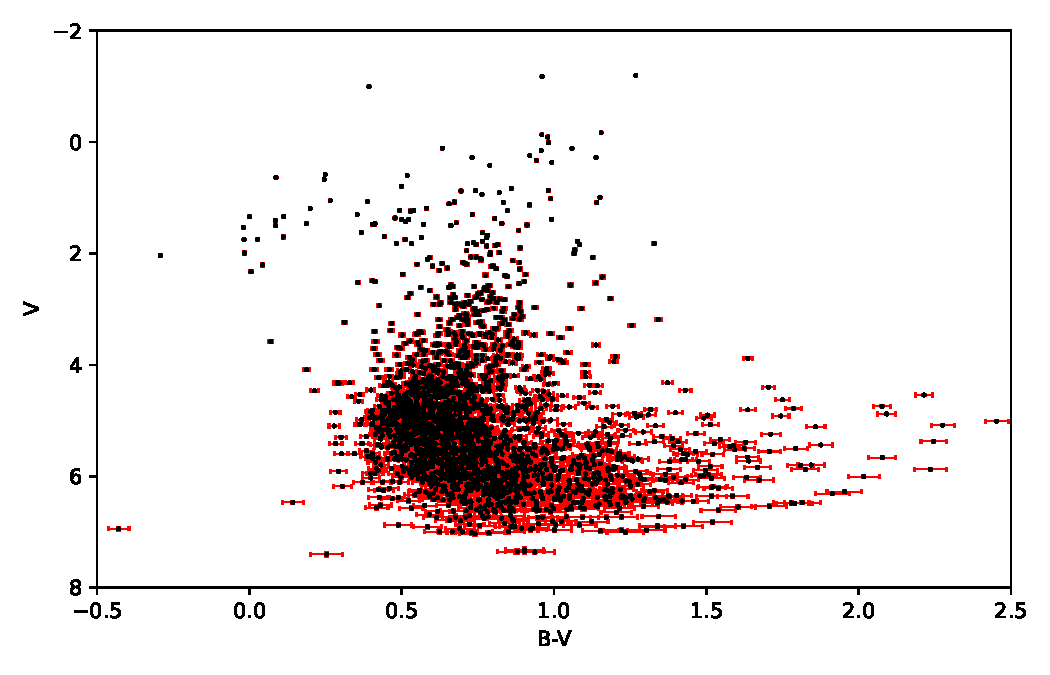
\includegraphics[width=0.8\textwidth]{../Figures/errobar}
	\caption{Colour magntiude diagram in the B and V filters from the matched dataset. The absulte magntiude in the V filter is shown on the y axis and the B magnitude minus V mangitude is shown on the x axis. Each data point has an error which is shown by the red error bars.}
	\label{fig:origin}
\end{figure}

To determine th

\begin{figure}
	\centering
	\begin{subfigure}[b]{0.49\textwidth}
		\centering
		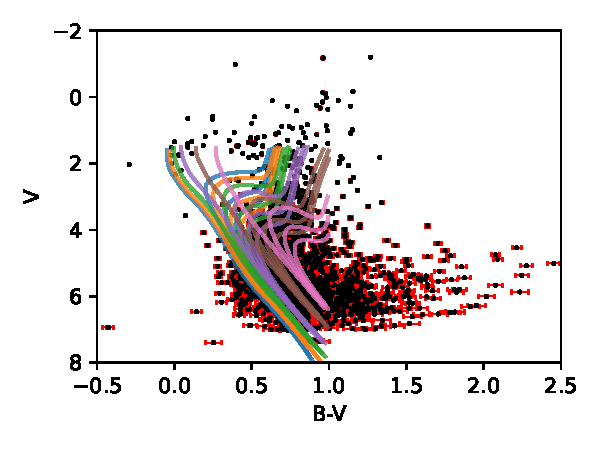
\includegraphics[width=\textwidth]{../Figures/manyiso}
		\caption{h}
		\label{fig:isomany}
	\end{subfigure}
	\hfill
	\begin{subfigure}[b]{0.49\textwidth}
		\centering
		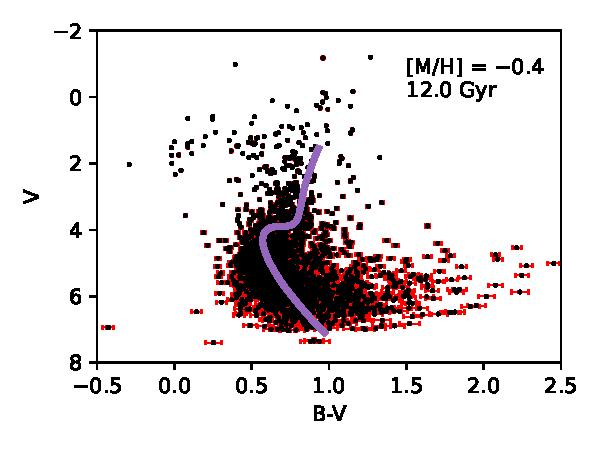
\includegraphics[width=\textwidth]{../Figures/singiso}
		\caption{h}
		\label{fig:singiso}
	\end{subfigure}
	\caption{}
	\label{fig:iso}
\end{figure}

\subsection{Spliting NGC 3201 into popultions based on distance from core}

\section{Discussion}

\section{Conclusion}

\bibliographystyle{agsm}
\bibliography{Mainref.bib}

\end{document}